%%%%%%%%%%%%%%%%%%%%%%%%%%%%%%%%%%%%%%%%%
% Beamer Presentation
% LaTeX Template
% Version 1.0 (10/11/12)
%
% This template has been downloaded from:
% http://www.LaTeXTemplates.com
%
% License:
% CC BY-NC-SA 3.0 (http://creativecommons.org/licenses/by-nc-sa/3.0/)
%
%%%%%%%%%%%%%%%%%%%%%%%%%%%%%%%%%%%%%%%%%

%----------------------------------------------------------------------------------------
%	PACKAGES AND THEMES
%----------------------------------------------------------------------------------------

\documentclass{beamer}

\mode<presentation> {

% The Beamer class comes with a number of default slide themes
% which change the colors and layouts of slides. Below this is a list
% of all the themes, uncomment each in turn to see what they look like.

%\usetheme{default}
%\usetheme{AnnArbor}
%\usetheme{Antibes}
%\usetheme{Bergen}
%\usetheme{Berkeley}
%\usetheme{Berlin}
%\usetheme{Boadilla}
%\usetheme{CambridgeUS}
%\usetheme{Copenhagen}
%\usetheme{Darmstadt}
%\usetheme{Dresden}
%\usetheme{Frankfurt}
%\usetheme{Goettingen}
%\usetheme{Hannover}
%\usetheme{Ilmenau}
%\usetheme{JuanLesPins}
%\usetheme{Luebeck}
\usetheme{Madrid}
%\usetheme{Malmoe}
%\usetheme{Marburg}
%\usetheme{Montpellier}
%\usetheme{PaloAlto}
%\usetheme{Pittsburgh}
%\usetheme{Rochester}
%\usetheme{Singapore}
%\usetheme{Szeged}
%\usetheme{Warsaw}

% As well as themes, the Beamer class has a number of color themes
% for any slide theme. Uncomment each of these in turn to see how it
% changes the colors of your current slide theme.

%\usecolortheme{albatross}
%\usecolortheme{beaver}
%\usecolortheme{beetle}
%\usecolortheme{crane}
%\usecolortheme{dolphin}
%\usecolortheme{dove}
%\usecolortheme{fly}
%\usecolortheme{lily}
%\usecolortheme{orchid}
%\usecolortheme{rose}
%\usecolortheme{seagull}
%\usecolortheme{seahorse}
%\usecolortheme{whale}
%\usecolortheme{wolverine}

%\setbeamertemplate{footline} % To remove the footer line in all slides uncomment this line
%\setbeamertemplate{footline}[page number] % To replace the footer line in all slides with a simple slide count uncomment this line

%\setbeamertemplate{navigation symbols}{} % To remove the navigation symbols from the bottom of all slides uncomment this line
}
\usepackage{graphicx} % Allows including images
\usepackage{booktabs} % Allows the use of \toprule, \midrule and \bottomrule in tables

\usepackage{array}

\usepackage{algorithm,algorithmic}
\usepackage{multicol}
\usepackage{caption,subcaption}
\usepackage{longtable}
\newcolumntype{V}[1]{>{\centering\arraybackslash} m{#1} }
\newcolumntype{L}[1]{>{\arraybackslash} m{#1} }

\pdfpageattr {/Group << /S /Transparency /I true /CS /DeviceRGB>>}%solves color issues brought by inserting pdf figures
%----------------------------------------------------------------------------------------
%	TITLE PAGE
%----------------------------------------------------------------------------------------

\title[Master Thesis Presentation]{An assistive handwashing system with emotional intelligence}
% The short title appears at the bottom of every slide, the full title is only on the title page

\author{Luyuan Lin} % Your name
\institute[UWaterloo] % Your institution as it will appear on the bottom of every slide, may be shorthand to save space
{
University of Waterloo \\ % Your institution for the title page
\medskip
\textit{Supervisor:
\newline Jesse Hoey
} % Your email address
}
\date{\today} % Date, can be changed to a custom date

\begin{document}

\begin{frame}
\titlepage % Print the title page as the first slide
\end{frame}

\begin{frame}
\frametitle{Agenda} % Table of contents slide, comment this block out to remove it
\tableofcontents % Throughout your presentation, if you choose to use \section{} and \subsection{} commands, these will automatically be printed on this slide as an overview of your presentation
\end{frame}

%----------------------------------------------------------------------------------------
%	PRESENTATION SLIDES
%----------------------------------------------------------------------------------------

%-----------------------------------------------------------------
\section{Problem Statement} 
% Sections can be created in order to organize your presentation into discrete blocks
% all sections and subsections are automatically printed in the table of contents as an overview of the talk
%------------------------------------------------
\subsection{Motivation}
\begin{frame}
\frametitle{Problem Statement - Motivation}
The COACH system
\begin{columns}[c]
\column{.5\textwidth}
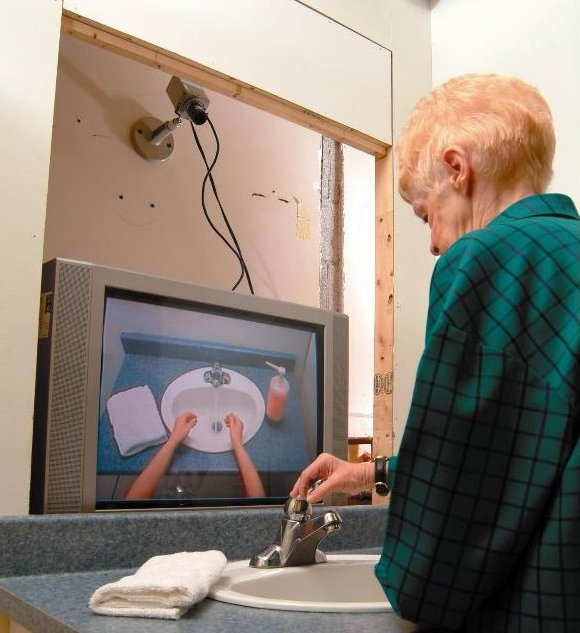
\includegraphics[width=\linewidth]{fig/testwash-flip.jpg}
\column{.5\textwidth}
\begin{itemize}
\item An assistive system helping people with dementia (e.g. Alzheimer's Disease) completing daily activities
\item Works well for some persons, but not as well for others
\item Only considers functional states of users
\end{itemize}
\end{columns}
\end{frame}

%------------------------------------------------
\subsection{Objectives}
\begin{frame}
\frametitle{Problem Statement - Objectives}
To augment the COACH system with an emotional reasoning engine so that the augmented system:\\
\begin{itemize}
\item is designed in a portable and extensible way
\item runs in real-time from the perspective of the user group
\item provides a level of functional assistance
\item produces the prompts according to the emotional state of a user
\end{itemize}
\vspace{.5cm}
Using Emotional Intelligence in Assitive Systems is the future direction.
\end{frame}

%-----------------------------------------------------------------
\section{Basic Concepts}
%------------------------------------------------
\subsection{Affect Control Theory (ACT)}
\begin{frame}
\frametitle{Concepts - ACT}
Affect Control Theory (ACT)
\begin{itemize}
\item represents emotions as EPA vectors, where E stands for ``evaluation'', P stands for ``potency'',
and A stands for ``activity''
\item describes social events by an Actor-Behaviour-Object grammar
\item ``fundamentals'' of identities and behaviours; shared between people within a same culture
\item ``transient impressions'': emotional feelings caused by a specific event
\end{itemize}
\pause
\begin{block}{The ACT Principle}
Actors work to experience transient impressions that are consistent with their fundamental sentiments.
\end{block}
\end{frame}

%------------------------------------------------
\subsection{The BayesACT Framework}
\begin{frame}
\frametitle{Concepts - BayesACT}
\begin{itemize}
\item A Bayesian version of the ACT theory
\item Extends the ACT with POMDP model
\item Uses a ``turn-taking'' model and represents state variables for Agent, Behaviour and Client (ABC)
\end{itemize}
%insert figure & explain the bayesact framework
\begin{columns}[c]
\column{.5\textwidth}
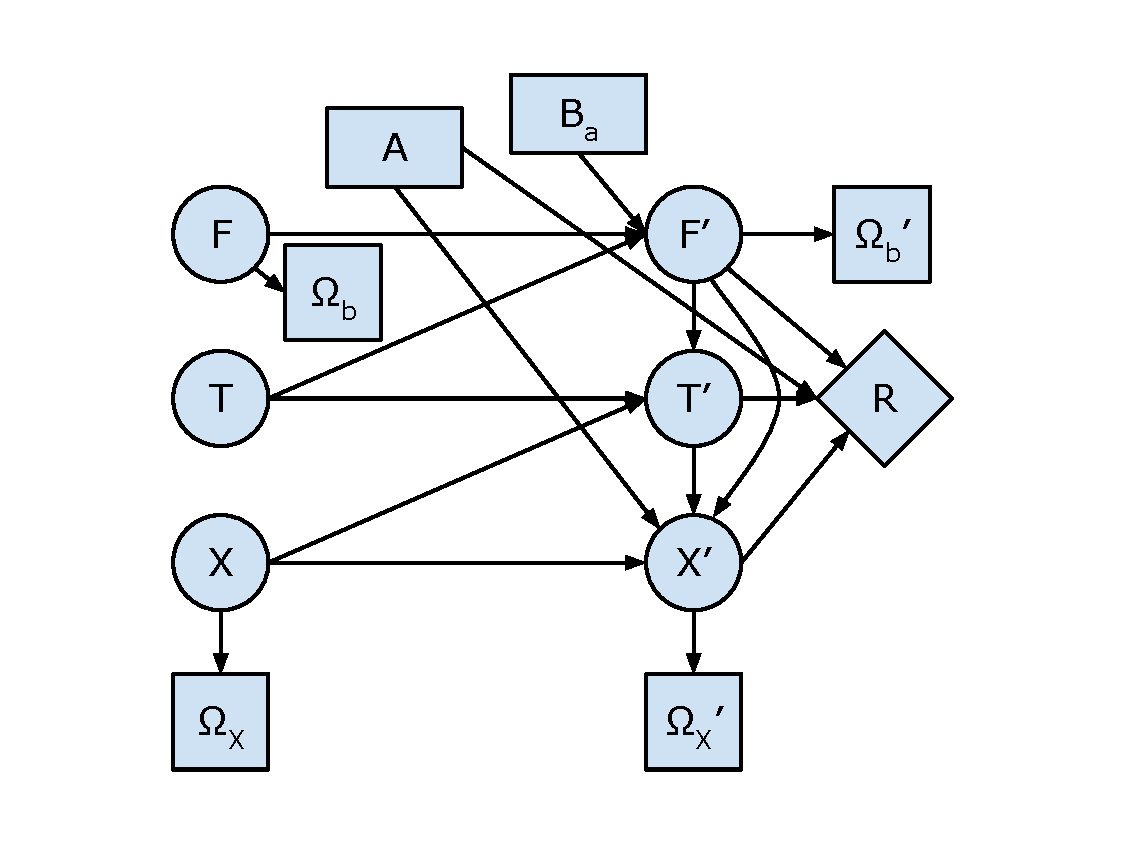
\includegraphics[trim = 20mm 10mm 20mm 10mm, clip, width=\linewidth]{fig/fig-bayesact.pdf}
\column{.5\textwidth}
\begin{itemize}
\item States $S = \{X, F, T\}$, where $F = \{F_{ij}\}, T = \{T_{ij}\}, i \in \{a, b, c\}, j \in \{e, p, a\}$
\item Note: $F_{c}$ denotes the agent's belief of the client's identity
\item Observations $\Omega = \{\Omega_{X}, \Omega_{b}\}$
\item Actions $\{A, B_{a}\}$
\item Calculate $\{A, B_{a}\}$ based on $\{X, F, T\}$
\end{itemize}
\end{columns}
\end{frame}


%-----------------------------------------------------------------
\section{System Design}
%------------------------------------------------

\begin{frame}
\frametitle{Design - Overview}
%insert figure describing the functionality of each component of the system
%state how each component is related to our objective
\begin{figure}
\centering
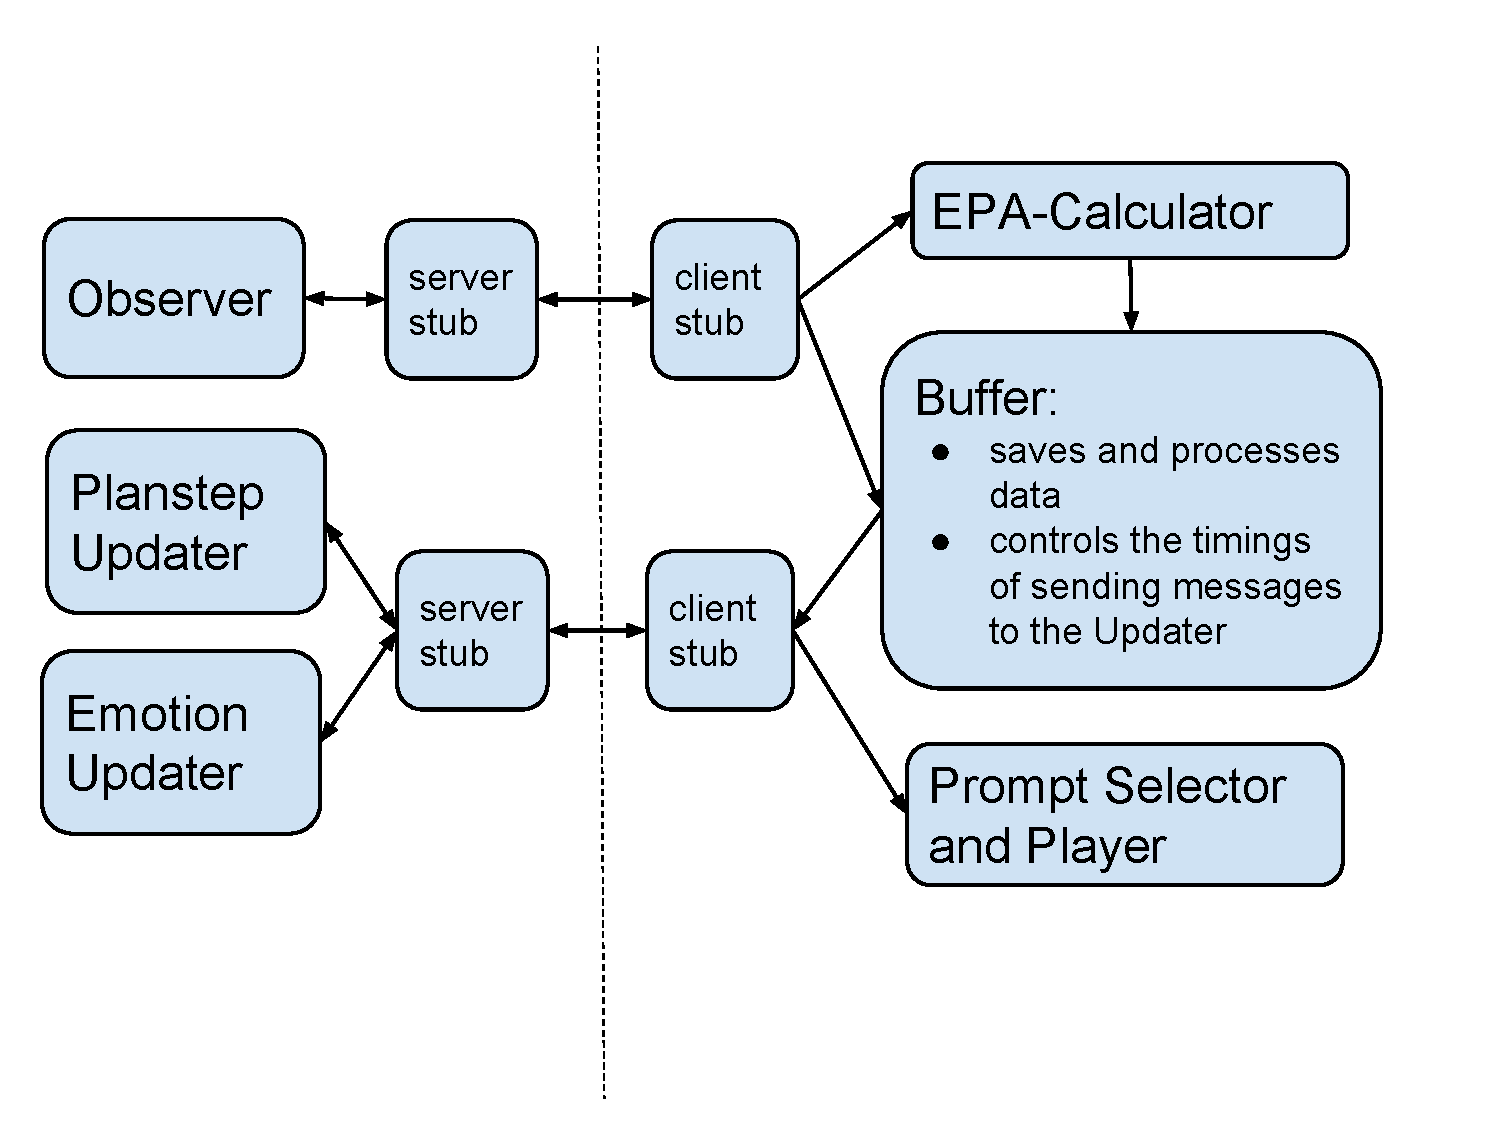
\includegraphics[trim = 5mm 15mm 5mm 20mm, clip, width=.8\linewidth]{fig/fig-system-overview.pdf}
\end{figure}
%state the server-client model is used & a "buffer" component is involved
%we focus on explaining how the servers is designed in "components" and then how they coordinate later
\end{frame}

%------------------------------------------------
\begin{frame}
\frametitle{Design - the Planstep and Emotion Updater}
%insert figure: the model & how emotional states are updated (explaining how the bayesact framework works in a specific app scenario)
%note: there's a noise parameter describing the confidence of a certain result
Use the BayesACT framework in the handwashing scenario
\begin{itemize}
\item Recall: BayesACT includes states $S = \{X, F, T\}$, observations $\Omega = \{\Omega_{x}, \Omega_{b}\}$, and agent actions $\{A, B_{a}\}$
\pause \item In our hand-washing system, $X = \{X_{turn}, X_{ps}, X_{aw}, X_{behav}\}$
\pause \item Observations give evidence to the state variables
\item Note: the ``confidence'' of $\Omega_b$ can be specified by $\gamma$, which is the variance of a normal (Gaussian) distribution.
\pause \item Compute $X_{ps}'$ based on $\Omega_{x}$, $\Omega_{b}$ and $\{X, F, T\}$
\pause \item Calculate $\{A, B_{a}\}$ based on $\{X, F, T\}$
\end{itemize}
\end{frame}

\begin{frame}
\frametitle{Design - the EPA-Calculator}
\begin{itemize}
\item Calculates affective meanings of user behaviours
%feature selection (other feature-selection approaches are not feasible in current situation)
\vspace{.3cm}
\item Feature Selection
\begin{itemize}
\item analysis on facial expressions and speeches?
\item related research for this special application scenario hasn't been done yet
\end{itemize}
%describe the threshold-based method (i.e. piecewise linear interpolation)
\pause
\vspace{.3cm}
\item Our approach
\begin{itemize}
\item $E$ stays neutral (value = 0); its value is ignored in the reasoning engine
\item $P$ scaled from the expansiveness of the user's two hands
\item $A$ scaled from the moving speeds of the user's hands
\item Used piecewise linear interpolation method
\end{itemize}
\vspace{.3cm}
\item ``Confidence'' of $\Omega_b$ can be specified in the reasoning engine
\end{itemize}
\end{frame}


\begin{frame}
\frametitle{Design - the Observer}
\begin{itemize}
%state how the original hand-tracker works
\item Step 1: Get the locations of the user's hands
\begin{itemize}
\item bases on a body tracker implemented in previous work
\item obtains locations of body parts from depth images taken from an overhead perspective
\item was trained using partially labeled, unbalanced data, and is configurable and re-trainable
\begin{figure}[htb]
\centering
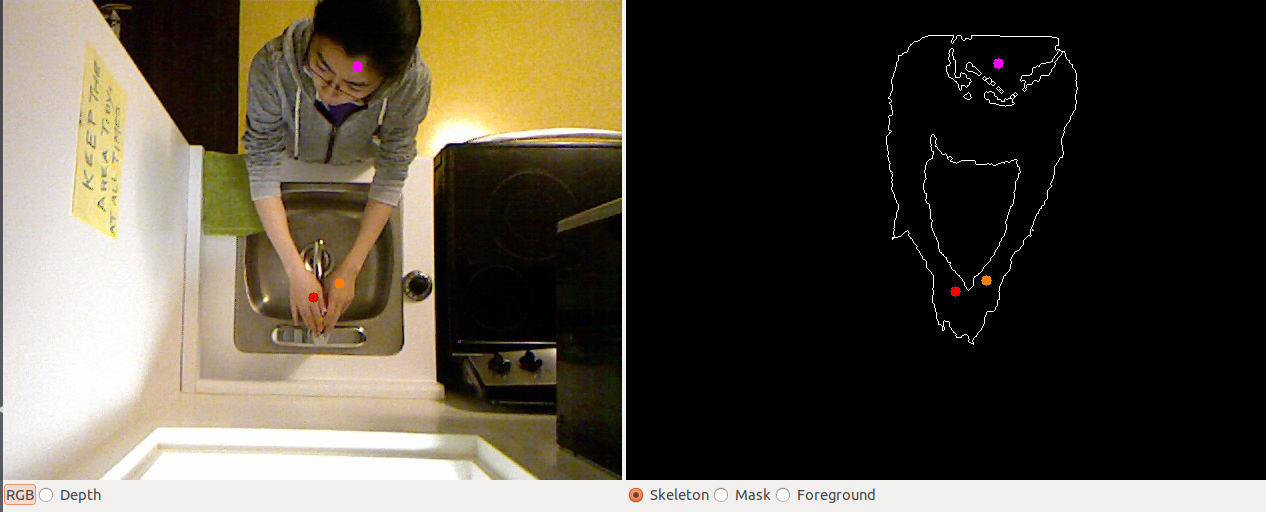
\includegraphics[width=0.9\linewidth]{fig/handtracker-performance.png}
\end{figure}
\end{itemize}
\end{itemize}
\end{frame}

\begin{frame}
\frametitle{Design - the Observer}
\begin{itemize}
\item Step 2: Map locations to user behaviours
\begin{itemize}
\item if hands are close to an object, then there's high probability of performing the behaviour corresponded to the object
\end{itemize}
\vspace{.3cm}
\item Observation noise handled by the observation function in the reasoning engine
\end{itemize}
\end{frame}

\begin{frame}
\frametitle{Design - the Prompt Selector and Player}
\begin{itemize}
%describe the survey - insert figure: examples of the prompts
\item The prompt dataset 
\begin{itemize}
\item 30 audio-visual prompts generated in previous study
\item created using the USC Virtual Human Toolkit
\item EPA values of videos evaluated by human raters
\end{itemize}
%figure: Screenshots of two video prompts stating same propositional messages
\begin{figure}[htb]
\centering
\begin{subfigure}[b]{.4\textwidth}
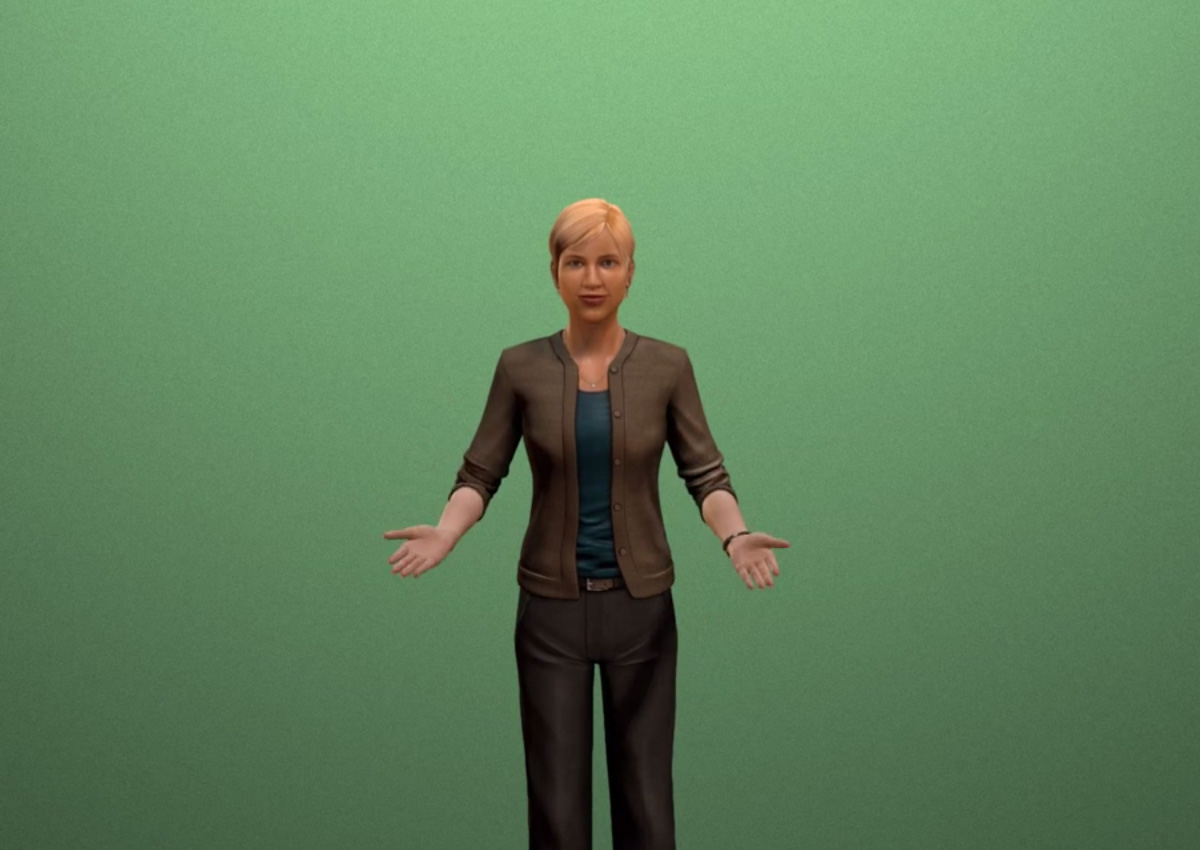
\includegraphics[width=\textwidth]{fig/prompt1.jpg}
\end{subfigure}
\begin{subfigure}[b]{.4\textwidth}
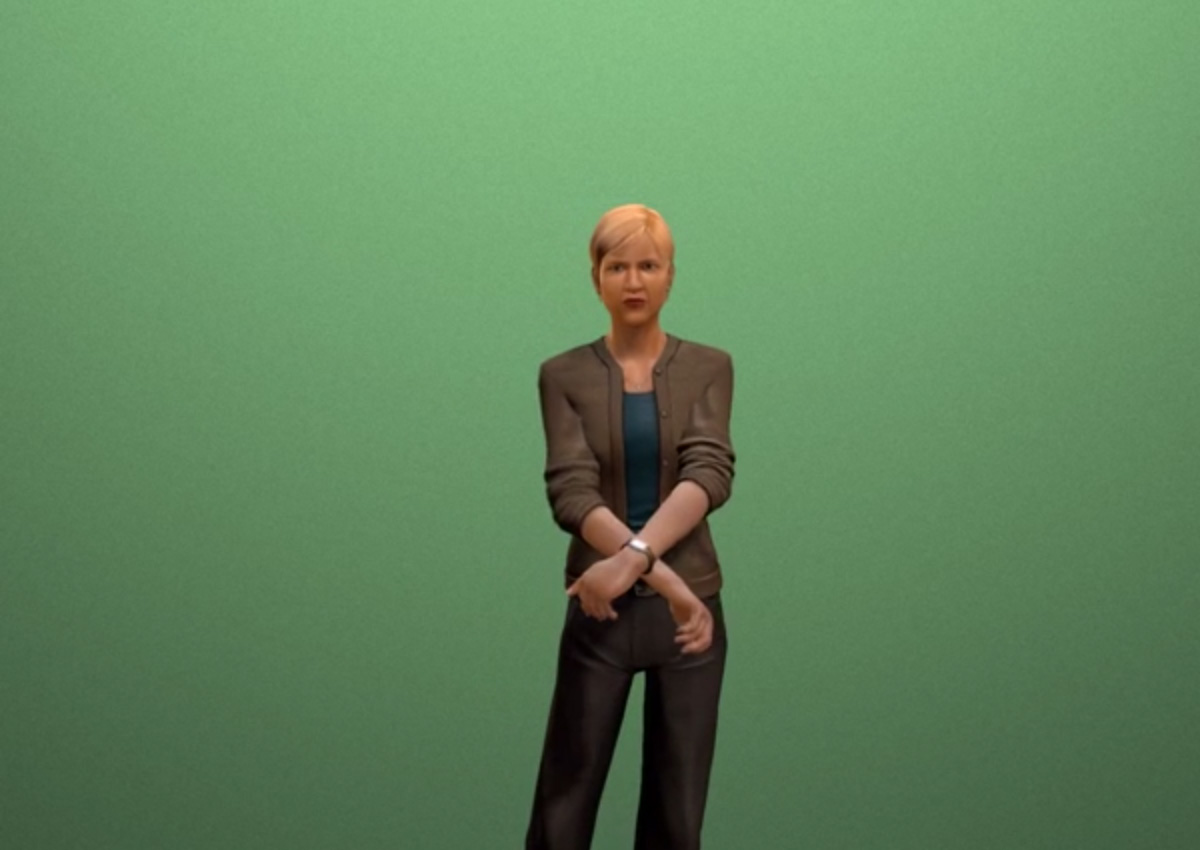
\includegraphics[width=\textwidth]{fig/prompt2.jpg}
\end{subfigure}
\end{figure}
%describe how to select (include formula defining the distance of prompts)
\item A proper prompt is selected as the final prompt if it:
\begin{itemize}
\item has the same propositional labels as the desired prompt
\item has the closest emotional (EPA) values as the desired prompt
\end{itemize}
\end{itemize}
\end{frame}

%-----------------------------------------------------------------
\section{Experimental Results}
%-----------------------------------------------------------
\begin{frame}
\frametitle{Experiments - Latency of the system}
Average latency of the system
\begin{itemize} 
\item 46.80ms for obtaining user behaviours
\item 1.65s for calculating and updating functional and emotional beliefs
\item 1.70s in total
\end{itemize}
\vspace{.3cm}
The system runs in real-time from the perspective of its user group
\end{frame}

\begin{frame}
\frametitle{Experiments - Two laboratory tests}
%what happened in the two runs
%explanation focus on planstep responses
%mention emotional responses in general
Two laboratory tests
\begin{itemize}
\item washed hands while the system observed and assisted in real time
\item acted more powerfully and more actively in the first test than the second
\item link to video of test \#2
\item results shown in thesis
\end{itemize}
\vspace{.3cm}
Another 15 tests were also run. Results are in the Appendix.
\end{frame}

\begin{frame}
\frametitle{Experiments - Conclusion}
%mention that more experiments were run & result is in the appendix 
\begin{itemize}
%planstep updater - they can update accordingly
\item Functionality performance
\begin{itemize}
\item sometimes false positively recognizes an user behaviour
\item in general, is able to produce propositionally useful system prompts
\end{itemize}
%emotion updater - insert table & state the correlations found between EPA values
\item Emotionality performance
% fig: Comparison of EPA values in the two tests
\begin{columns}[c]
\column{.6\textwidth}
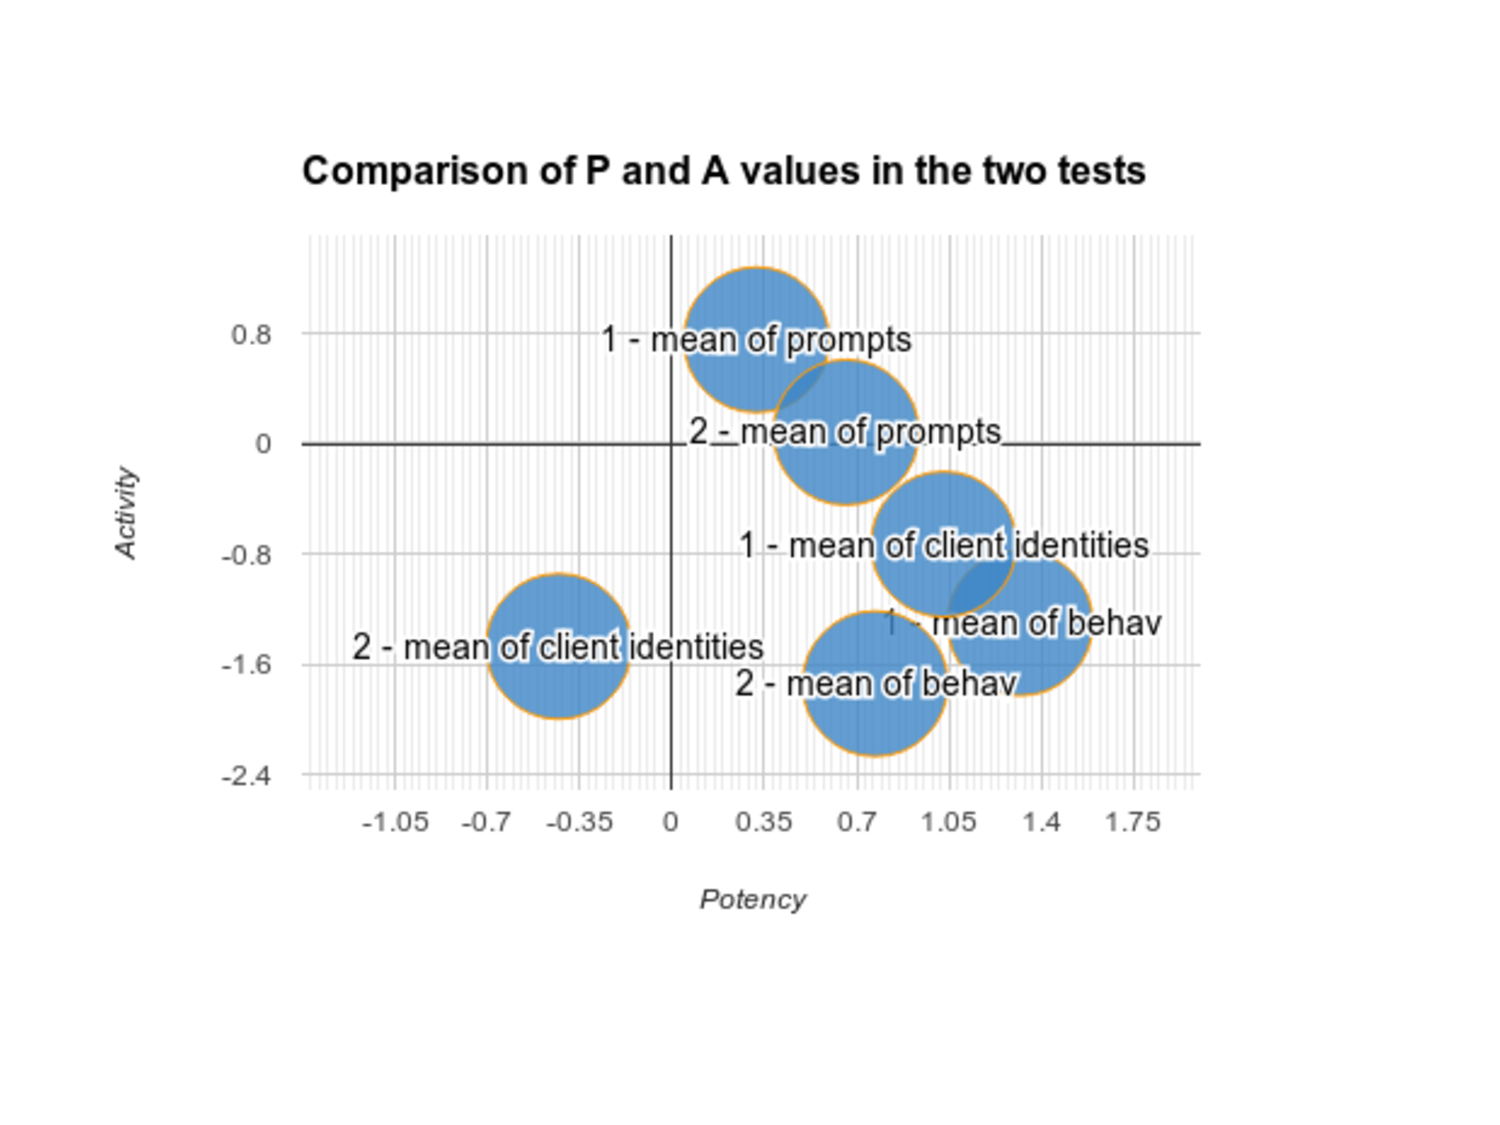
\includegraphics[trim=10mm 45mm 25mm 10mm, clip, width=\linewidth]{fig/fig-compare-two-tests.pdf}
\column{.45\textwidth}
Generally, user behaviours with higher $P$ and higher $A$ values lead to
\begin{itemize}
\item client identities with higher $P$ and higher $A$ values
\item system prompts with lower $P$ and higher $A$ values
\item as predicted by the Affect Control Theory
\end{itemize}
\end{columns}
\end{itemize}
\end{frame}

%-----------------------------------------------------------------
\section{Discussion}
%-----------------------------------------------------------

\begin{frame}
\frametitle{Discussion}
%state contribution of this paper
Contribution
\begin{itemize}
\item Designed and implemented a prototypical hand-washing system that satisfies the objectives
\item Tests also indicated a correlation between the EPA values of user behaviours, user identities, and system prompts
\end{itemize}
\vspace{.3cm}
Future Work
\begin{itemize}
\item{Improve the EPA-Calculator}
\item{Improve the prompt generation process}
\item{Improve the Planstep- and Emotion- Updater}
\item{Conduct clinical trials for the system}
\end{itemize}
\end{frame}

%---------------------------------------------------------------
% Ending pages
%---------------------------------------------------------------
\begin{frame}
\frametitle{Acknowledgement}
This work is based on previous works of:
\begin{itemize}
\footnotesize{
\item Hoey, J., Schroder, T., \& Alhothali, A. (2013, September). Bayesian affect control theory. In Affective Computing and Intelligent Interaction (ACII), 2013 Humaine Association Conference on (pp. 166-172). IEEE.
\item Czarnuch, S., \& Mihailidis, A. (2014 (in review)). Depth image hand tracking from an overhead perspective using partially labeled, unbalanced data: Development and real-world testing. IEEE Journal of Biomedical and Health Informatics.
\item Malhotra, A., Yu, C., Schr¨oder, T., \& Hoey, J. (2014 (in review)). An exploratory study into the use of an emotionally aware cognitive assistant.
}
\end{itemize}
\vspace{0.3cm}
I'd like to take this opportunity to thank:
\begin{itemize}
\item Jesse Hoey
\item James Tung and Peter van Beek
\item Stephen Czarnuch, Aarti Malhotra and Celia Yu
\item Families and friends, especially Chengbo Li, Xiao Yang, Enxun Wei and Luyi Lin
\end{itemize}
\end{frame}
%------------------------------------------------
\begin{frame}
\frametitle{The end}
\Huge{\centerline{Thank you!}}   
\fontsize{5mm}{4mm}
\begin{itemize}
\item Questions?
\item Comments?
\end{itemize}
\end{frame}
%----------------------------------------------------------------------------------------

%---------------------------------------------------------------
% Additional pages
% put pages in assistance to answering questions here
%---------------------------------------------------------------

\begin{frame}
\frametitle{Concepts - BayesACT cont.}
Model formulation
\begin{itemize}
% ---- formula computing deflection ----
\item The deflection $\phi(F, T)$ between $F$ and $T$: 
\begin{equation}\label{eq:eq_deflection}
\phi(f,t) \propto e^{-(f'-t')\Sigma^{-1}(f-t)}
\end{equation}
% ---- formula computing probability of $f'$ ----
\item The probability of a post-action fundamental sentiment $f'$:
\begin{equation}\label{eq:eq_pr_f}
Pr(f'|f,t,x,b_{a},\phi) \propto e^{-\phi(f',t')-\xi(f',f,b_{a},x)} 
\end{equation}
where $t'$ can be computed from $\{f', t, x\}$ by empirically derived prediction equations of ACT.
% ---- how the application progresses (i.e. how planstep changes in our case) ----
\item $Pr(x'|x,f',t',a)$: how the application progresses
% ---- observation functions ----
\item $Pr(\omega_{b}|f)$ and $Pr(\omega_{x}|x)$: observation functions for the client behaviour sentiment and system state 
\end{itemize}
\end{frame}

%pseudo-code page(1): how planstep is updated according to behavioural obs, awareness, & deflection
\begin{frame}
\frametitle{Update $X_{ps}'$ based on $\Omega_{x}$ and $\{X_{ps}, X_{behav}, X_{aw}, F, T\}$}
\begin{itemize}
\item $SampleXVar()$ and $evalSampleXVar()$
\item Pseudocode of $SampleXVar()$ (on next page)
\item $Pr: X_{behav} \to \Delta(\Omega_{x})$ used in $evalSampleXVar()$
\end{itemize}
\end{frame}

%pseudo-code page(2): how planstep is updated according to behavioural obs, awareness, & deflection
\begin{frame}
\frametitle{Update $X_{ps}'$ based on $\Omega_{x}$ and $\{X_{ps}, X_{behav}, X_{aw}, F, T\}$ cont.}
%----------------- second item -----------------
\algsetup{linenosize=\scriptsize}
\begin{algorithm}[H]
\scriptsize
\begin{multicols}{2}
\begin{algorithmic}[1]
\IF {Deflection(F, T) is high} \STATE {
  threshold = high
} \ELSE \STATE {
  threshold = low
} \ENDIF
\IF {aw high} {
  \IF {prompted} {
    \IF{$random\_prob() <$ threshold} \STATE {
       aw = low and not moving forward
    } \ELSIF {prompt wrong} \STATE {
       aw = low and not moving forward
    } \ELSIF {likely} \STATE {
       moving forward
    } \ELSIF {$random\_prob() <$ threshold} \STATE {
       aw = low and not moving forward
    } \ENDIF
  } \ELSE {
    \IF {$random\_prob() <$ threshold} \STATE {
      aw = low and not moving forward
    } \ELSE \STATE {
      aw stays high and moving forward
    } \ENDIF
  } \ENDIF
} \ELSE {
  \IF {prompted} {
    \IF {$random\_prob() >$ threshold \AND prompt correct} \STATE {
	move on and aw high
    } \ELSE \STATE {
        unlikely: aw high and not moving forward
    } \ENDIF
  } \ELSE \STATE {
      unlikely: aw high and moving forward
  } \ENDIF
} \ENDIF
\end{algorithmic}
% compile k
\end{multicols}
\end{algorithm}
\end{frame}

%------------------------------------------------
\begin{frame}
\frametitle{Concepts - POMDP}
Partially Observable Markov Decision Process (POMDP)
\vspace{.3cm}
\begin{columns}[c]
\column{.5\textwidth}
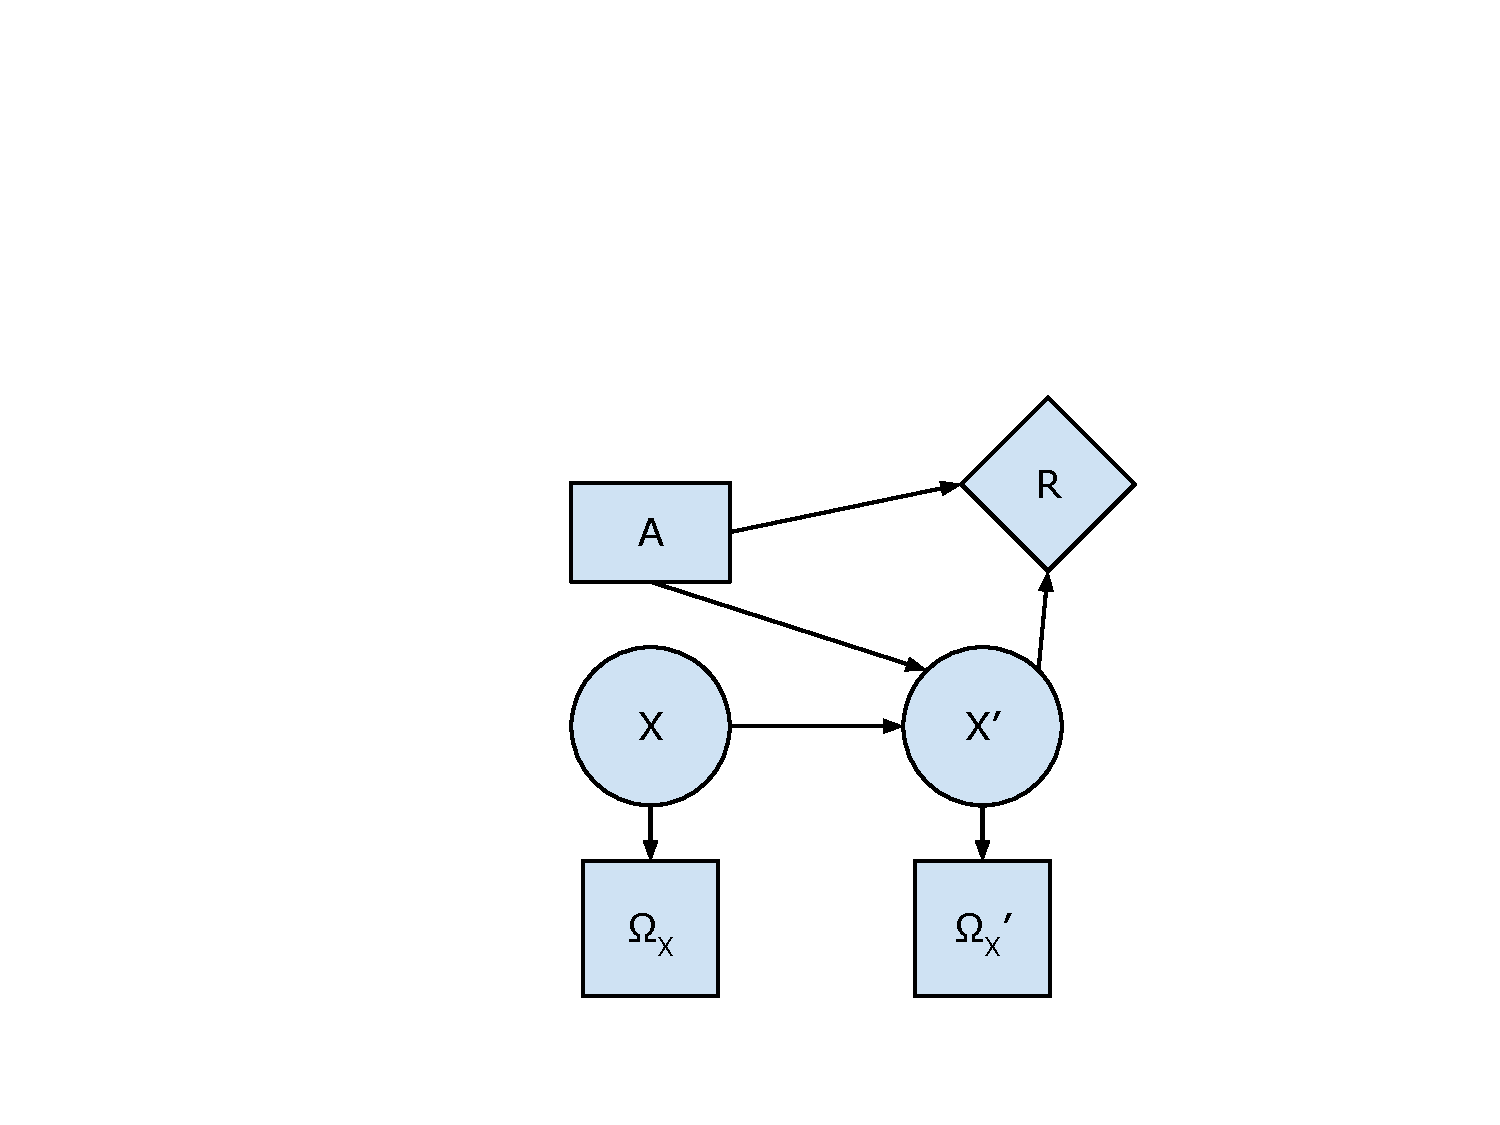
\includegraphics[trim = 45mm 20mm 30mm 50mm, clip, width=\textwidth]{fig/fig-pomdp-simple.pdf}
\column{.5\textwidth}
\begin{itemize}
\item A timeslice of a POMDP process
\item Variables: \{ $X$, $A$, $\mathbf{\Omega_{X}}$ \}
\item $Pr : X \to \Delta(\mathbf{\Omega_{X}})$, $Pr : X \times A \to \Delta(\mathbf{X})$
\item Reward Function: $R(A, X')$
\end{itemize}
\end{columns}
\end{frame}


%------------------------------------------------
\begin{frame}
\frametitle{Solution - Representing ``Functional States''}
%planstep definitions: the 8 ps & 5 behaviours monitored
Planstep Definition and Update Diagram
\begin{figure}[htp]
\centering
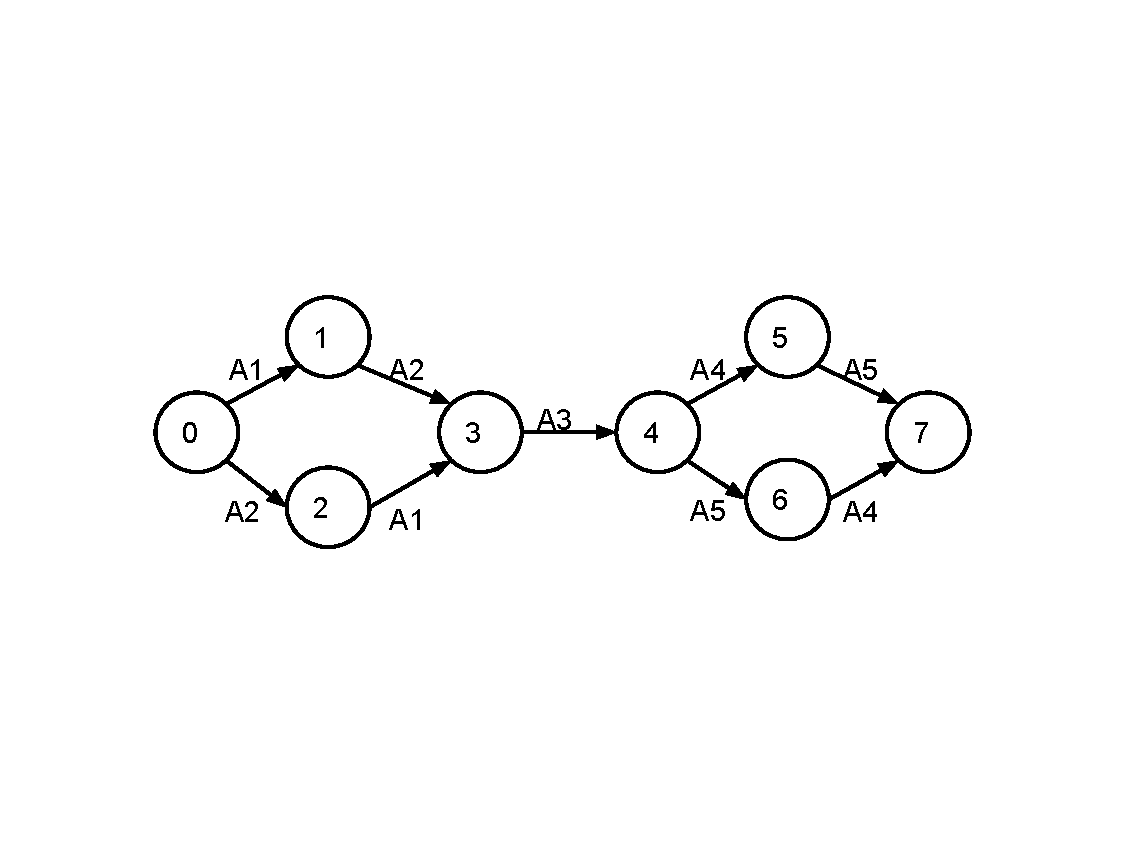
\includegraphics[trim = 20mm 50mm 20mm 50mm, clip, width=0.8\textwidth]{fig/fig-planstep.pdf}
\label{fig:planstep}
\end{figure}
\begin{itemize}
\item Eight plansteps: (0) ``off/dirty/dry'', (1) ``on/dirty/dry'', (2) ``off/soapy/dry'', (3) ``on/soapy/dry'', (4) ``on/clean/wet'', (5) ``off/clean/wet'', (6) ``on/clean/dry'', (7) ``off/clean/dry''
\item Five behaviours: A1 to A5 are ``turn on water'', ``put on soap'', ``rinse hands'', ``turn off water'', and ``use towel'', respectively.
\end{itemize}
\end{frame}


%------------------------------------------------
\begin{frame}
\frametitle{Solution - The Buffer}
\begin{itemize}
\item Between the Observer, the EPA-Calc, and the Reasoning Engine
\item Controls timings of sending messages
\begin{figure}
\centering
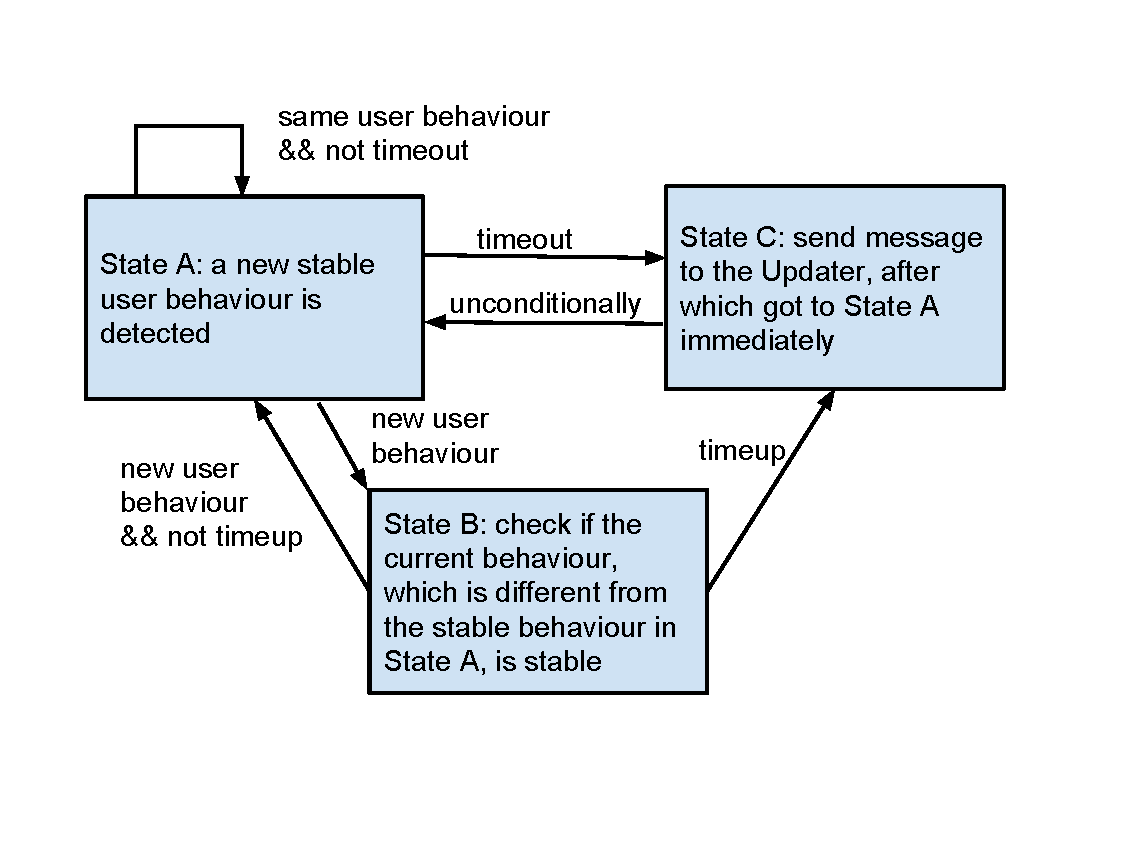
\includegraphics[trim = 10mm 25mm 16mm 15mm, clip, width=0.75\linewidth]{fig/fig-state-trans.pdf}
\end{figure}
\item Smoothes EPA values calucated by the Calculator
\end{itemize}
\end{frame}

%------------------------------------------------
\begin{frame}
\frametitle{Experiments - Parameter values used in laboratory experiments}
%table: Parameter values used in laboratory experiments - explain the meanings of all the parameters
\begin{table}
\small
\centering
\begin{tabular}{| l | l | l |}
\hline
\textbf{Param.} & \textbf{Value} & \textbf{Defined in which component} \\ \hline
$n$ & $10$ & EPA-Calc \\ \hline
$distance$ & $\{-\infty, 0, 8, 40, 128, 160, +\infty\}$ & EPA-Calc \\ \hline
$potency$ & $\{-4.3, -4.3, 0, 1, 2, 4.3, 4.3\}$ & EPA-Calc  \\ \hline 
$difference$ & $\{-\infty, 0, 3.5, 17.5, 35, 70, +\infty\}$ & EPA-Calc \\ \hline
$activity$ & $\{-4.3, -4.3, -2, -1, 0, 4.3, 4.3\}$ & EPA-Calc\\ \hline
$alpha$ & $0$ & Buffer \\ \hline
$timeout$ & $300$ & Buffer \\ \hline
$timeup$ & $1$ & Buffer \\ \hline
$\beta_{a}^{0}$ & $0.001$ & Updater \\ \hline
$\beta_{c}^{0}$ & $2.0$ & Updater \\ \hline
$\gamma$ & $(100000, 1.0, 0.5)$ & Updater\\ \hline
$N$ & $2000$ & Updater \\ \hline
$f_a^{0}$ & $[1.5, 0.51, 0.45]$ & Updater \\ \hline
$f_c^{0}$ & Different in each test &Updater \\ \hline
\end{tabular}
\end{table}
\end{frame}


\end{document} 
